\documentclass{standalone}

\usepackage[x11names]{xcolor}
\usepackage{tikz}

\begin{document}

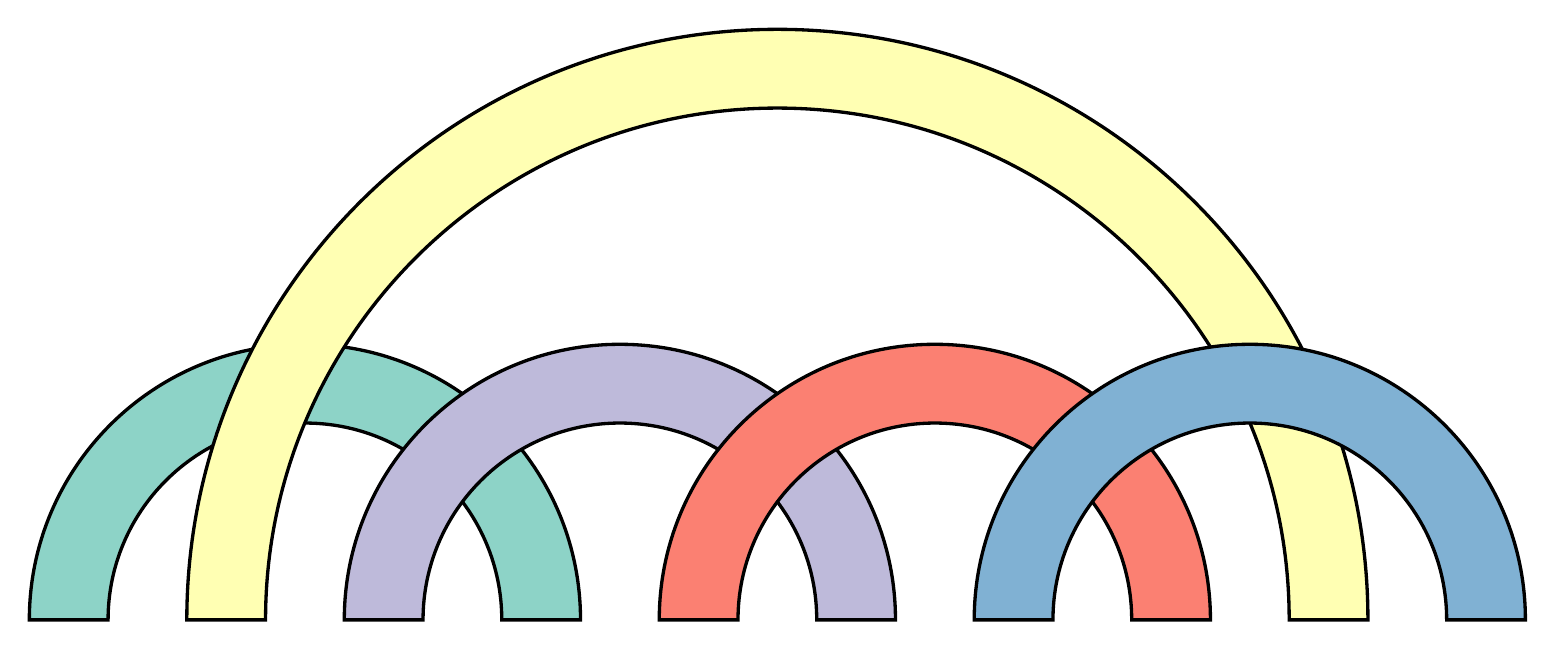
\begin{tikzpicture}

\definecolor{c1}{rgb}{0.5529411764705883, 0.8274509803921568, 0.7803921568627451}
\definecolor{c2}{rgb}{1.0, 1.0, 0.7019607843137254}
\definecolor{c3}{rgb}{0.7450980392156863, 0.7294117647058823, 0.8549019607843137}
\definecolor{c4}{rgb}{0.984313725490196, 0.5019607843137255, 0.4470588235294118}
\definecolor{c5}{rgb}{0.5019607843137255, 0.6941176470588235, 0.8274509803921568}

\filldraw[very thick, fill=c1] (0,0) arc (180:0:3.5) -- (6,0) arc (0:180:2.5) -- cycle;
\filldraw[very thick, fill=c2] (2,0) arc (180:0:7.5) -- (16,0) arc (0:180:6.5) -- cycle;
\filldraw[very thick, fill=c3] (4,0) arc (180:0:3.5) -- (10,0) arc (0:180:2.5) -- cycle;
\filldraw[very thick, fill=c4] (8,0) arc (180:0:3.5) -- (14,0) arc (0:180:2.5) -- cycle;
\filldraw[very thick, fill=c5] (12,0) arc (180:0:3.5) -- (18,0) arc (0:180:2.5) -- cycle;

\end{tikzpicture}


\end{document}
